\documentclass{article}

% 导入宏包
\usepackage{fancyhdr}
\usepackage{ctex}
\usepackage{listings}
\usepackage{graphicx}
\usepackage[a4paper, body={18cm,22cm}]{geometry}
\usepackage{amsmath,amsthm,amssymb,amstext,wasysym,enumerate,graphicx}
\usepackage{float,abstract,booktabs,indentfirst,amsmath}
\usepackage{array}
\usepackage{multirow}
\usepackage{url}
\usepackage{diagbox}
\usepackage{enumitem}
\usepackage{xcolor}
\usepackage{makecell}
\usepackage{tikz}
\usepackage{tcolorbox}
\usetikzlibrary{positioning, arrows.meta}
\usepackage[bookmarks=true, colorlinks, citecolor=blue, linkcolor=black]{hyperref}


% 设置段落
\renewcommand\arraystretch{1.4}
\setlength{\parindent}{2em}
\setCJKmonofont{黑体}

% 设置高亮文字
\newtcbox{\mybox}[1][red]
{on line, arc = 0pt, outer arc = 0pt,
	colback = #1!10!white, colframe = #1!50!black,
	boxsep = 0pt, left = 1pt, right = 1pt, top = 2pt, bottom = 2pt,
	boxrule = 0pt, bottomrule = 1pt, toprule = 1pt}

% 配置代码显示
\lstset{
	xleftmargin = 3em,
	xrightmargin = 3em,
	aboveskip = 1em,
	backgroundcolor = \color{white},
	basicstyle = \small\ttfamily,
	rulesepcolor = \color{gray},
	breaklines = true,
	numbers = left,
	numberstyle = \small,
	numbersep = -14pt,
	keywordstyle = \color{purple}\bfseries,
	commentstyle = \color{green!60!black}, % 修改注释颜色
	stringstyle = \color{red!60!green!90!blue!90},
	morekeywords = {ASSERT, int64_t, uint32_t},
	moreemph = {ASSERT, NULL},
	emphstyle = \color{red}\bfseries,
	moreemph = [2]{int64\_t, uint32\_t, tid\_t, uint8\_t, int16\_t, uint16\_t, int32\_t, size\_t, bool},
	emphstyle = [2]\color{purple}\bfseries,
	frame = shadowbox,
	showspaces = false,
	columns = fixed
	morecomment = [l][\color{green!60!black}]{+}, % 设置以+开头的代码行为绿色
}

%--------------------页眉--------------------%

\pagestyle{fancy}
\fancyhead[L]{}
\fancyhead[R]{}
\fancyhead[C]{华东师范大学软件工程学院实验报告}
\fancyfoot[C]{-\thepage-}
\renewcommand{\headrulewidth}{1.5pt}

%--------------------标题--------------------%

\begin{document}
	\begin{center}
		{\Large{\textbf{\heiti 华东师范大学软件工程学院实验报告}}}
		\begin{table}[htb]
			\flushleft
			\begin{tabular}{p{0.4\linewidth}p{0.27\linewidth}p{0.28\linewidth}}\\
				\textbf{实验课程}:数据库系统及其应用实践  & \textbf{年级}:2023级       & \textbf{实验成绩}:  \\
				\textbf{实验名称}:Lab-01 & \textbf{姓名}:顾翌炜         &                 \\
				\textbf{实验编号}:Lab-01     & \textbf{学号}:10235101527 & \textbf{实验日期}:2025/03/06  \\
				\textbf{指导教师}:姚俊杰     & \textbf{组号}:01            & \textbf{实验时间}:2课时  \\ 
			\end{tabular}
		\end{table}
	\end{center}
	\rule{\textwidth}{2pt}
	
	\begin{tcolorbox}[title = {备注}, colback = blue!25!white, colframe = blue!75!black]
		在基于college的task2中,涉及到很多name相同,id却不同的学生的问题,考虑到其中的2000个id无一重复,而name却有432个重复,显得有些不合理,所以相关问题我都用了两种方法来回答(一种是\textbf{distinct ID}, 一种是\textbf{distinct name})两种方法在我的报告里都会有展示
	\end{tcolorbox}
	
    \section{实验目标}
    
    学习和熟悉使用\texttt{SQL}查询语句
    
    \section{实验要求}
    
    \begin{enumerate}[noitemsep, label={{\arabic*})}]
    	\item 按照实验内容,依次完成每个实验步骤;
    	
    	\item 操作实验步骤时,需要理解该操作步骤的目的,预判操作的结果;当操作结果与预判不符时,及时向任课教师和助教咨询;
    	
    	\item 在实验报告中依次记录主要操作步骤的内容和结果(返回的消息或截图);
    	
    	\item 对实验中遇到的问题、解决方案及收获进行总结;
    	
    	\item 确保实验报告整洁、美观(注意字体、字号、对齐、截图大小和分页等;)
    	
    \end{enumerate}\textbf{}
    
    \section{实验过程记录}
    
    \subsection{安装sql环境以及数据库的集成开发环境}
    
    按照老师提供的文档安装sql环境并配置,安装方法略
    
    \subsection{新建数据库并运行sql文件}
    
    在DataGrip中新建一个数据库并测试连接
    
    \begin{figure}[H]
    	\centering
    	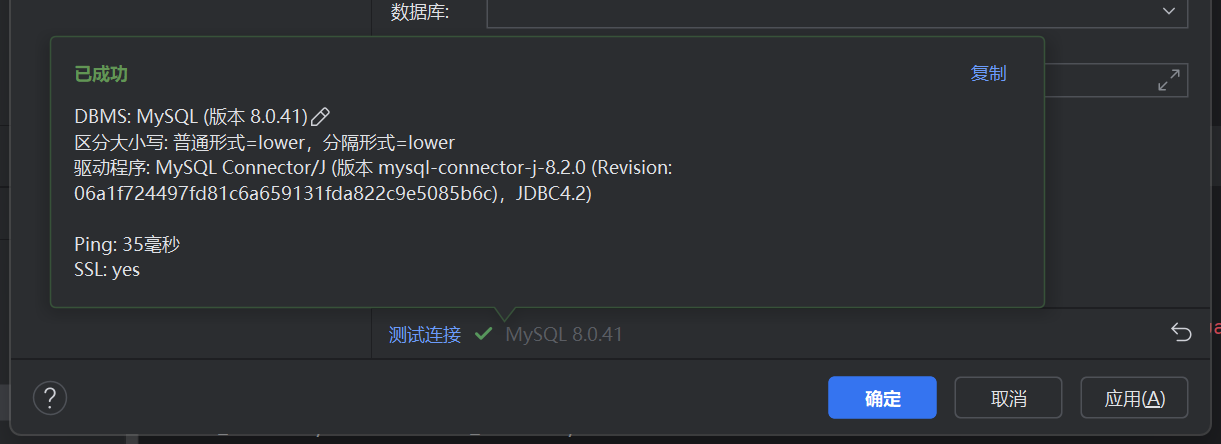
\includegraphics[width=10cm]{./images/1.测试连接.png}
    	\caption{测试连接}
    \end{figure}
    
    运行Lab-01文件夹内的\textbf{activity.sql}和\textbf{college.sql}文件完成实验的环境创建。
    
    \subsection{Task 1 - based on database activity}
    
    通过观察\textbf{activity.sql}可以发现:
    
    \begin{lstlisting}[language=sql, title=activity.sql, tabsize=4]
    -- ----------------------------
    -- Table structure for activity
    -- ----------------------------
    CREATE TABLE `activity`  (
    `actid` int NOT NULL,
    `activity_name` varchar(25) CHARACTER SET utf8mb4 COLLATE utf8mb4_0900_ai_ci NULL DEFAULT NULL,
    PRIMARY KEY (`actid`) USING BTREE
    ) ENGINE = InnoDB CHARACTER SET = utf8mb4 COLLATE = utf8mb4_0900_ai_ci ROW_FORMAT = Dynamic;
    
    -- ----------------------------
    -- Table structure for faculty
    -- ----------------------------
    CREATE TABLE `faculty`  (
    `FacID` int NOT NULL,
    `Lname` varchar(15) CHARACTER SET utf8mb4 COLLATE utf8mb4_0900_ai_ci NULL DEFAULT NULL,
    `Fname` varchar(15) CHARACTER SET utf8mb4 COLLATE utf8mb4_0900_ai_ci NULL DEFAULT NULL,
    `_Rank` varchar(15) CHARACTER SET utf8mb4 COLLATE utf8mb4_0900_ai_ci NULL DEFAULT NULL,
    `Sex` char(1) CHARACTER SET utf8mb4 COLLATE utf8mb4_0900_ai_ci NULL DEFAULT NULL,
    `Phone` int NULL DEFAULT NULL,
    `Room` char(5) CHARACTER SET utf8mb4 COLLATE utf8mb4_0900_ai_ci NULL DEFAULT NULL,
    `Building` varchar(13) CHARACTER SET utf8mb4 COLLATE utf8mb4_0900_ai_ci NULL DEFAULT NULL,
    PRIMARY KEY (`FacID`) USING BTREE
    ) ENGINE = InnoDB CHARACTER SET = utf8mb4 COLLATE = utf8mb4_0900_ai_ci ROW_FORMAT = Dynamic;
    
    
    -- ----------------------------
    -- 以下省略,共五张表格
    -- ----------------------------
    \end{lstlisting}
    
    可以看出\textbf{activity}中表格的列如下所示:
    
    \begin{tcolorbox}[title = {\textbf{activity}的表格}, colback = blue!25!white, colframe = blue!75!black]
    	\textbf{activity} (actid, activity\_name) \\
    	\textbf{faculty} (FacID, Lname, Fname, \_Rank, Sex, Phone, Room, Building) \\
    	\textbf{faculty\_participate\_in} (FacID, actid) \\
    	\textbf{participate\_in} (stuid, actid) \\
    	\textbf{student} (StuID, LName, Fname, Age, Sex, Major, Advisor, city\_code)
    \end{tcolorbox}
    
    为了更清晰的展现数据库中外键等关系,可以用下图形式展现:
    
    \begin{figure}[H]
    	\centering
    	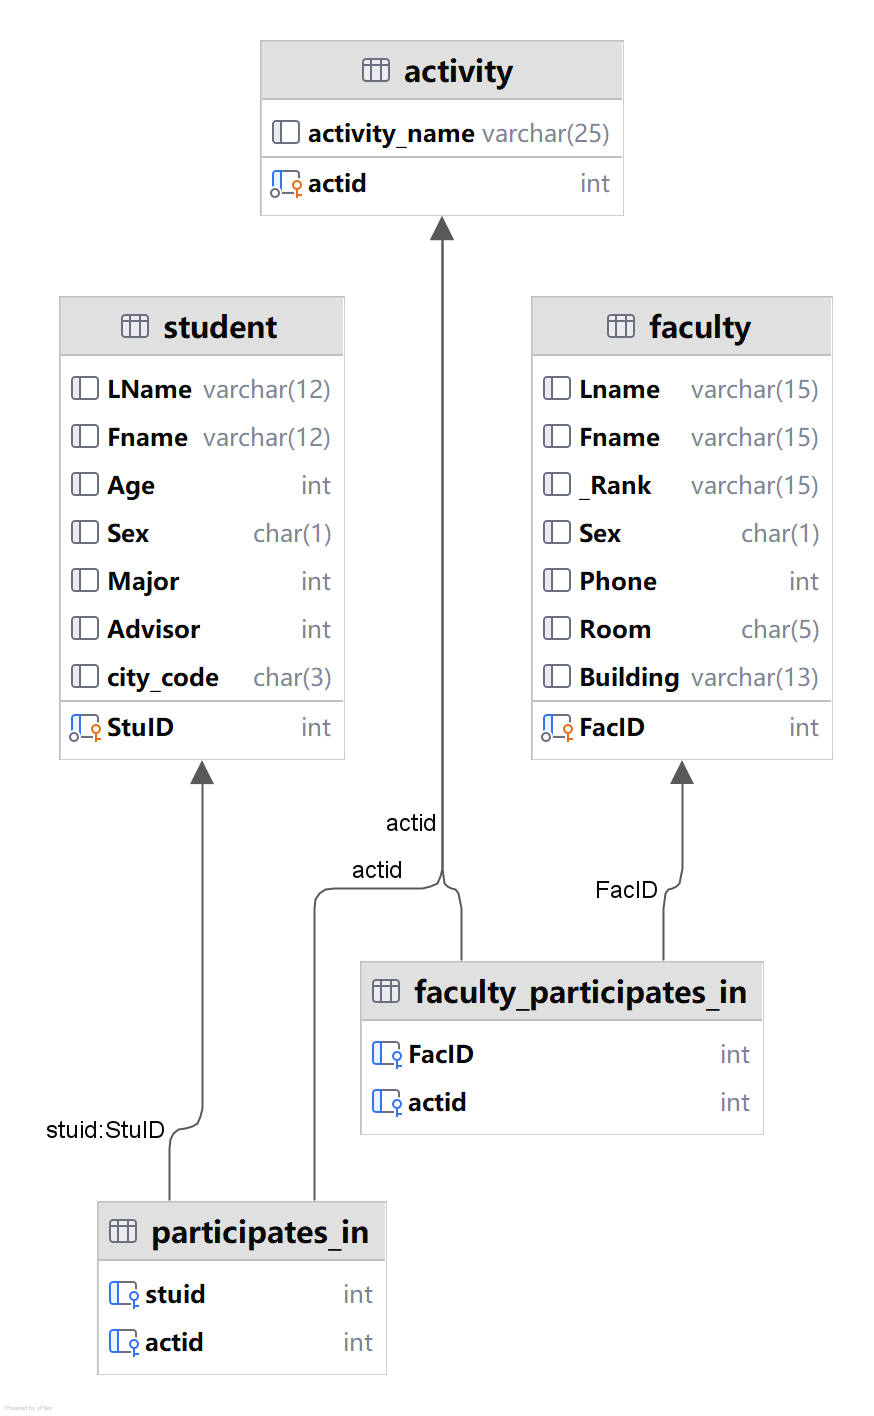
\includegraphics[width=6cm]{./images/2.activity关系.png}
    	\caption{activity关系}
    \end{figure}
    
    \subsubsection{Queation 0}
    
    Give me the number of faculty members who participate in an activity  (easy)
    
    \begin{lstlisting}[language=sql, title=Queation 0, tabsize=4]
    	select count(distinct faculty.FacID)
    	from faculty,
    		faculty_participates_in
    	where faculty.FacID = faculty_participates_in.FacID;
    \end{lstlisting}
    
    运行结果入下图所示:
    
    \begin{figure}[H]
    	\centering
    	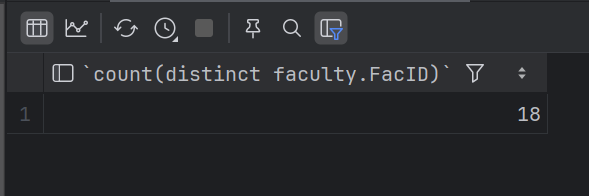
\includegraphics[width=7cm]{./images/3.Question 0.png}
    	\caption{Question 0}
    \end{figure}
    
    得到的结果是:18
    
    \subsubsection{Queation 1}
    
    How many activities do we have?  (easy)
    
    \begin{lstlisting}[language=sql, title=Queation 1, tabsize=4]
    	select count(actid)
    	from activity;
    \end{lstlisting}
    
    运行结果入下图所示:
    
    \begin{figure}[H]
    	\centering
    	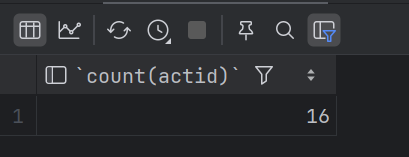
\includegraphics[width=7cm]{./images/4.Question1.png}
    	\caption{Question 1}
    \end{figure}
    
    得到的结果是:16
    
    \subsubsection{Question 2}
    
    How many faculty members does each building have? List the result with the name of the building.  (medium)
    
    \begin{lstlisting}[language=sql, title=Question 2, tabsize=4]
    	select Building, count(FacID)
    	from faculty
    	group by Building;
    \end{lstlisting}
    
    运行结果如下图所示:
    
    \begin{figure}[H]
    	\centering
    	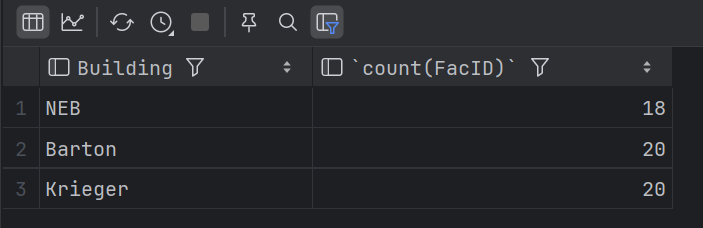
\includegraphics[width=9cm]{./images/5.Question2.png}
    	\caption{Question 2}
    \end{figure}
    
    得到的结果是:
    \begin{itemize}
    	\item NEB, 18
    	\item Barton, 20
    	\item Krieger, 20
    \end{itemize}
    
    \subsubsection{Question 3}
    
    How many activities does Mark Giuliano participate in?  (medium)
    
    \begin{lstlisting}[language=sql, title=Question 3, tabsize=4]
    	select count(faculty_participates_in.actid)
    	from faculty_participates_in,
    		 faculty
    	where faculty_participates_in.FacID = faculty.FacID
    	  and faculty.Fname = 'Mark'
    	  and faculty.Lname = 'Giuliano';
    \end{lstlisting}
    
    运行结果如下图所示:
    
    \begin{figure}[H]
    	\centering
    	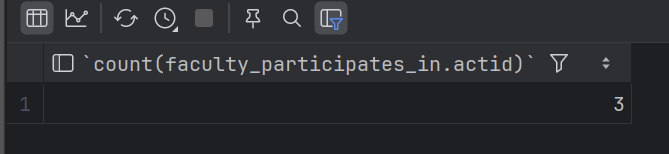
\includegraphics[width=9cm]{./images/6.Question3.png}
    	\caption{Question 3}
    \end{figure}
    
    得到的结果是:3
    
    \subsubsection{Question 4}
    
    Show the ids of the faculty who don't participate in any activity.  (hard)
    
    \begin{lstlisting}[language=sql, title=Question 4, tabsize=4]
    	select distinct faculty.FacID
    	from faculty,
    	faculty_participates_in
    	where faculty.FacID not in (select distinct faculty.FacID
    								from faculty,
    									 faculty_participates_in
    								where faculty.FacID = faculty_participates_in.FacID);
    \end{lstlisting}
    
    运行结果如下图所示:
    
    \begin{figure}[H]
    	\centering
    	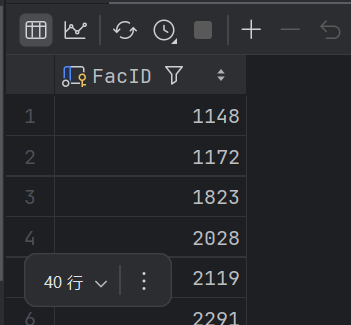
\includegraphics[width=7cm]{./images/7.Question4.png}
    	\caption{Question 4}
    \end{figure}
    
    得到的结果是:1148, 1172, 1823等40个元组
    
    \subsubsection{Question 5}
    
    What are the ids of the faculty members who do not advise any student?  (hard)
    
    \begin{lstlisting}[language=sql, title=Question 5, tabsize=4]
    	select FacID
    	from faculty
    	where FacID not in (select distinct Advisor
    						from student);
    \end{lstlisting}
    
    运行结果如下图所示:
    
    \begin{figure}[H]
    	\centering
    	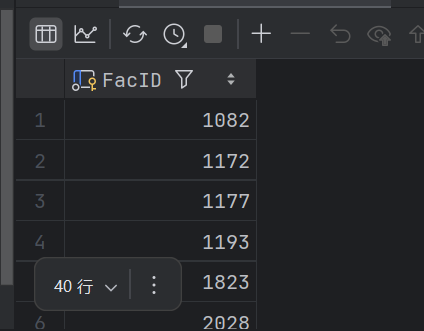
\includegraphics[width=7cm]{./images/8.Question5.png}
    	\caption{Question 5}
    \end{figure}
    
    得到的结果是:1082, 1172, 1177等40个元组
    
    \subsubsection{Question 6}
    
    Find the name of the activity that has the largest number of student participants.  (extra)
    
    \begin{lstlisting}[language=sql, title=Question 6, tabsize=4]
    	select activity_name
    	from (select activity_name, count(activity.actid)
    		  from activity,
    		  	   participates_in
    		  where activity.actid = participates_in.actid
    		  group by activity_name
    		  order by count(activity.actid) desc
    		  limit 1) as activity_count;
    \end{lstlisting}
    
    运行结果如下图所示:
    
    \begin{figure}[H]
    	\centering
    	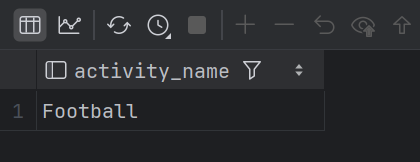
\includegraphics[width=7cm]{./images/9.Question6.png}
    	\caption{Question 6}
    \end{figure}
    
    得到的结果是:Football
    
    \subsubsection{Question 7}
    
    What are the first name and last name of Linda Smith's advisor?  (extra)
    
    \begin{lstlisting}[language=sql, title=Question 7, tabsize=4]
    	select faculty.Fname, faculty.LName
    	from faculty
    	where FacID = (select student.Advisor
    				   from student
    				   where Fname = 'Linda'
    				     and LName = 'Smith');
    \end{lstlisting}
    
    运行结果如下图所示:
    
    \begin{figure}[H]
    	\centering
    	
\includegraphics[width=9cm]{./images/10.Question7.png}
    	\caption{Question 7}
    \end{figure}
    
    得到的结果是:Michael, Goodrich
    
    \subsubsection{Question 8}
    
    Give me the first and last name of the faculty who advises the most students.  (extra)
    
    \begin{lstlisting}[language=sql, title=Question 8, tabsize=4]
    	select faculty.Fname, faculty.Lname
    	from faculty
    	where faculty.FacID = (select student.Advisor
    						   from student
    						   group by student.Advisor
    						   order by count(student.StuID) desc
    						   limit 1);
    \end{lstlisting}
    
    运行结果如下图所示:
    
    \begin{figure}[H]
    	\centering
    	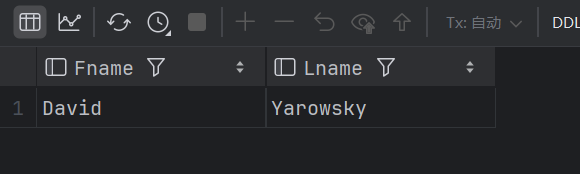
\includegraphics[width=9cm]{./images/11.Question8.png}
    	\caption{Question 8}
    \end{figure}
    
    得到的结果是:David, Yarowsky
    
    \subsubsection{Question 9}
    
    Find the ids of the students who participate in Canoeing and Kayaking.  (extra)
    
    \begin{lstlisting}[language=sql, title=Question 9, tabsize=4]
    	select distinct s.StuID
    	from student s
    	where s.StuID in (select s1.StuID
    				      from student s1,
    					  	   participates_in,
    					  	   activity
    					  where s1.StuID = participates_in.stuid
    						and participates_in.actid = activity.actid
    						and activity.activity_name = ('Canoeing'))
    						and s.StuID in (select s2.StuID
    					  from student s2,
    						   participates_in,
    						   activity
    					  where s2.StuID = participates_in.stuid
    						and participates_in.actid = activity.actid
    						and activity.activity_name = ('Kayaking'))
    \end{lstlisting}
    
    运行结果如下图所示:
    
    \begin{figure}[H]
    	\centering
    	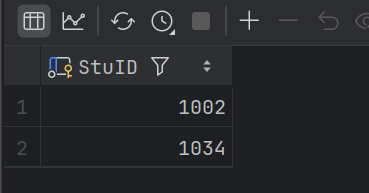
\includegraphics[width=7cm]{./images/12.Question9.png}
    	\caption{Question 9}
    \end{figure}
    
    得到的结果是:
    \begin{itemize}
    	\item 1002
    	\item 1034
    \end{itemize}
    
    \subsection{Task 2 - based on database college}
    
    通过观察\textbf{college.sql}可以发现:
    
    \begin{lstlisting}[language=sql, title=activity.sql, tabsize=4]
    	-- ----------------------------
    	-- Table structure for advisor
    	-- ----------------------------
    	DROP TABLE IF EXISTS `advisor`;
    	CREATE TABLE `advisor`  (
    	`s_ID` varchar(5) CHARACTER SET utf8mb4 COLLATE utf8mb4_0900_ai_ci NOT NULL,
    	`i_ID` varchar(5) CHARACTER SET utf8mb4 COLLATE utf8mb4_0900_ai_ci NULL DEFAULT NULL,
    	PRIMARY KEY (`s_ID`) USING BTREE,
    	INDEX `i_ID`(`i_ID` ASC) USING BTREE,
    	CONSTRAINT `advisor_ibfk_1` FOREIGN KEY (`i_ID`) REFERENCES `instructor` (`ID`) ON DELETE SET NULL ON UPDATE RESTRICT,
    	CONSTRAINT `advisor_ibfk_2` FOREIGN KEY (`s_ID`) REFERENCES `student` (`ID`) ON DELETE CASCADE ON UPDATE RESTRICT
    	) ENGINE = InnoDB CHARACTER SET = utf8mb4 COLLATE = utf8mb4_0900_ai_ci ROW_FORMAT = Dynamic;
    	
   	
    	-- ----------------------------
    	-- 以下省略,共11张表格
    	-- ----------------------------
    \end{lstlisting}
    
    可以看出\textbf{college}中表格的列如下所示:
    
    \begin{tcolorbox}[title = {\textbf{ER Diagram 表格}}, colback = blue!25!white, colframe = blue!75!black]
    	\textbf{department} (building, budget, dept\_name) \\
    	\textbf{course} (course\_id, title, dept\_name, credits) \\
    	\textbf{classroom} (building, room\_number, capacity) \\
    	\textbf{prereq} (course\_id, prereq\_id) \\
    	\textbf{section} (course\_id, sec\_id, semester, year, building, room\_number, time\_slot\_id) \\
    	\textbf{instructor} (ID, name, dept\_name, salary) \\
    	\textbf{student} (ID, name, dept\_name, tot\_cred) \\
    	\textbf{time\_slot} (time\_slot\_id, day, start\_hr, start\_min, end\_hr, end\_min) \\
    	\textbf{teaches} (ID, course\_id, sec\_id, semester, year) \\
    	\textbf{takes} (ID, course\_id, sec\_id, semester, year, grade) \\
    	\textbf{advisor} (s\_ID, i\_ID)
    \end{tcolorbox}
    
    
    为了更清晰的展现数据库中外键等关系,可以用下图形式展现:
    
    \begin{figure}[H]
    	\centering
    	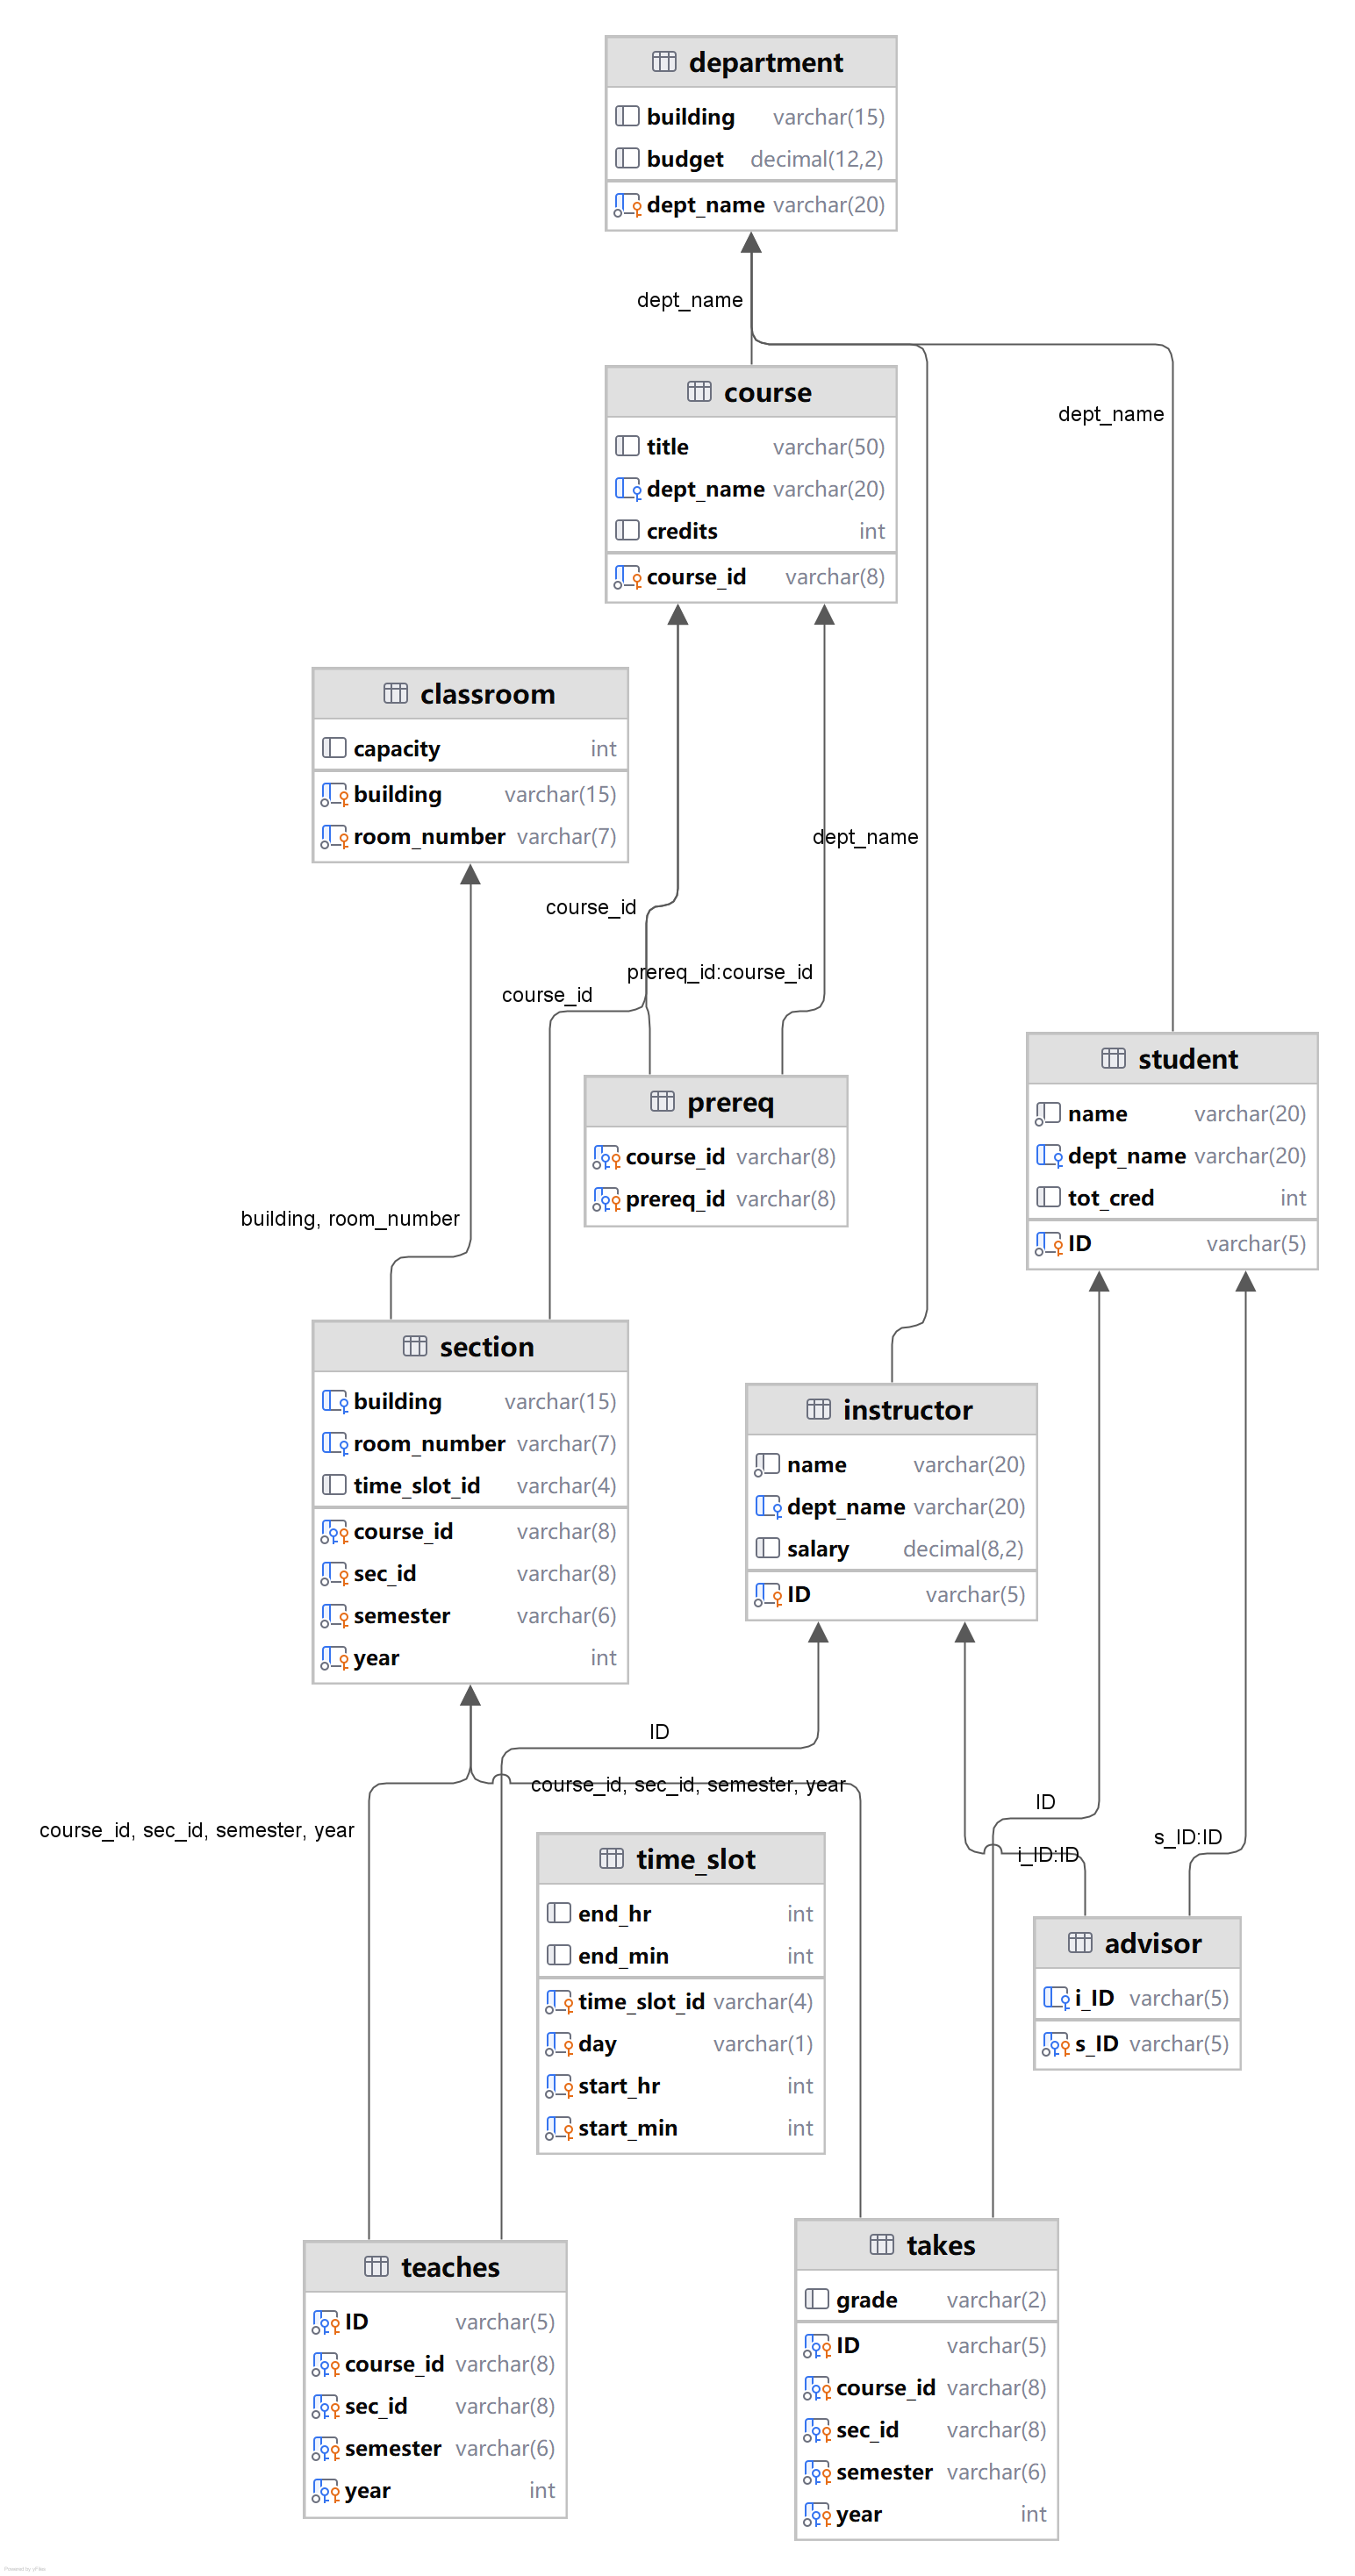
\includegraphics[width=10cm]{./images/13.college关系.png}
    	\caption{activity关系}
    \end{figure}
    
    \subsubsection{Question 10}
    
    List the names of all courses ordered by their titles and credits.  (easy)
    
    \begin{lstlisting}[language=sql, title=Question 10, tabsize=4]
    	select title
    	from course
    	order by title, credits;
    \end{lstlisting}
    
    运行结果如下图所示:
    
    \begin{figure}[H]
    	\centering
    	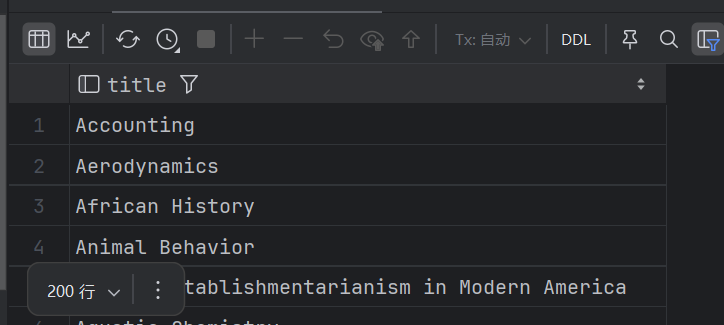
\includegraphics[width=9cm]{./images/14.Question10.png}
    	\caption{Question 10}
    \end{figure}
    
    得到的结果是:Accounting, Aerodynamics等200个元组
    
    \subsubsection{Question 11}
    
    Count the number of students who have advisors.  (easy)
    
    答案1:\mybox[blue]{假设相同的name表示同一个学生}
    
    \begin{lstlisting}[language=sql, title=Question 11, tabsize=4]
    	select count(distinct student.name)
    	from student
    			join advisor
    				on student.ID = advisor.s_ID
    					and i_ID is not null;
    \end{lstlisting}
    
    运行结果如下图所示:
    
    \begin{figure}[H]
    	\centering
    	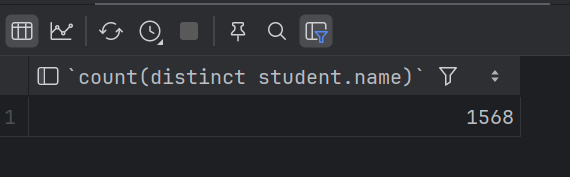
\includegraphics[width=7cm]{./images/15.Question11-ans1.png}
    	\caption{Question 11}
    \end{figure}
    
    得到的结果是:1568
    
    \mybox[red]{备注:由于本题涉及到了id没有重复值,name却有432个重复值的问题,所以本题上传第二种答案}
    
    答案2:\mybox[blue]{假设相同的id表示同一个学生}
    
    \begin{lstlisting}[language=sql, title=Question 11, tabsize=4]
    	select count(distinct student.ID)
    	from student
    			join advisor
    				on student.ID = advisor.s_ID
    					and i_ID is not null;
    \end{lstlisting}
    
    运行结果如下图所示:
    
    \begin{figure}[H]
    	\centering
    	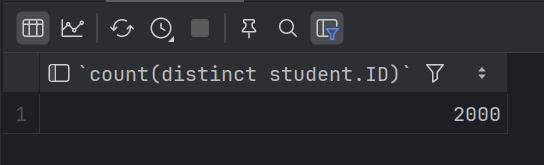
\includegraphics[width=7cm]{./images/15.Question11-ans2.png}
    	\caption{Question 11}
    \end{figure}
    
    得到的结果是:2000
    
    \subsubsection{Question 12}
    
    How many departments offer courses?  (easy)
    
    \begin{lstlisting}[language=sql, title=Question 12, tabsize=4]
    	select count(distinct course.dept_name)
    	from course;
    \end{lstlisting}
    
    运行结果如下图所示:
    
    \begin{figure}[H]
    	\centering
    	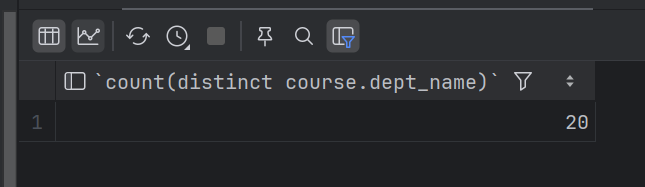
\includegraphics[width=7cm]{./images/16.Question12.png}
    	\caption{Question 12}
    \end{figure}
    
    得到的结果是:20
    
    \subsubsection{Question 13}
    
    List the information of all instructors ordered by their salary in ascending order.  (easy)
    
    \begin{lstlisting}[language=sql, title=Question 13, tabsize=4]
    	select *
    	from instructor
    	order by salary;
    \end{lstlisting}
    
    运行结果如下图所示:
    
    \begin{figure}[H]
    	\centering
    	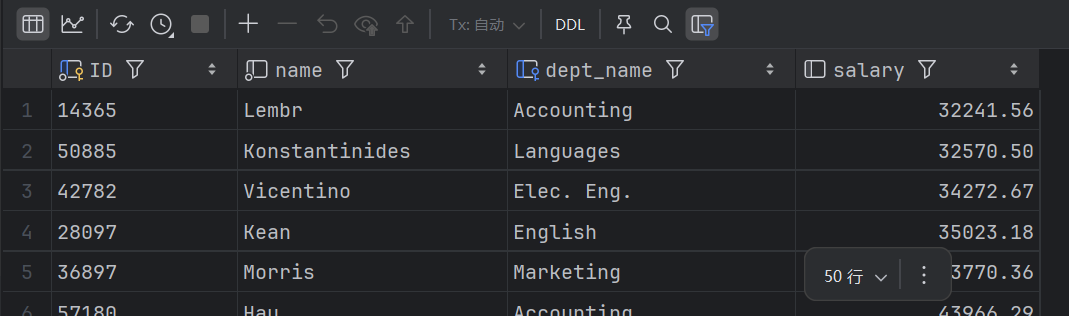
\includegraphics[width=10cm]{./images/17.Question13.png}
    	\caption{Question 13}
    \end{figure}
    
    得到的结果是:(14365, Lembr, Accounting, 32241.56
    )等50个元组
    
    \subsubsection{Question 14}
    
    How many different courses offered by Physics department? (easy)
    
    \begin{lstlisting}[language=sql, title=Question 14, tabsize=4]
    	select count(course.title)
    	from course
    	where dept_name = 'Physics';
    \end{lstlisting}
    
    运行结果如下图所示:
    
    \begin{figure}[H]
    	\centering
    	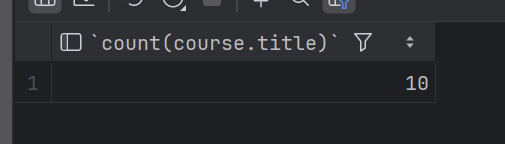
\includegraphics[width=7cm]{./images/18.Question14.png}
    	\caption{Question 14}
    \end{figure}
    
    得到的结果是:10
    
    \subsubsection{Question 15}
    
    What are the titles for courses with two prerequisites? (medium)
    
    \begin{lstlisting}[language=sql, title=Question 15, tabsize=4] 
    	select title 
    	from course 
    		join prereq 
    			on course.course_id = prereq.course_id 
    	group by course.course_id 
    	having count(prereq_id) = 2; 
    \end{lstlisting}
    
    运行结果如下图所示:
    
    \begin{figure}[H] 
    	\centering 
    	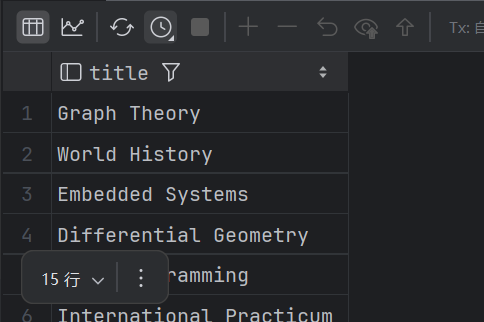
\includegraphics[width=7cm]{./images/19.Question15.png} 
    	\caption{Question 15} 
    \end{figure}
    
    得到的结果是:Graph Theory, World History等15个元组
    
    \subsubsection{Question 16}
    
    What is the title, credit value, and department name for courses with more than one prerequisite?  (medium)
    
    \begin{lstlisting}[language=sql, title=Question 16, tabsize=4]
    	select title, credits, dept_name
    	from course
    			join prereq
    				on course.course_id = prereq.course_id
    	group by title, credits, dept_name
    	having count(prereq_id) > 1;
    \end{lstlisting}
    
    运行结果如下图所示:
    
    \begin{figure}[H]
    	\centering
    	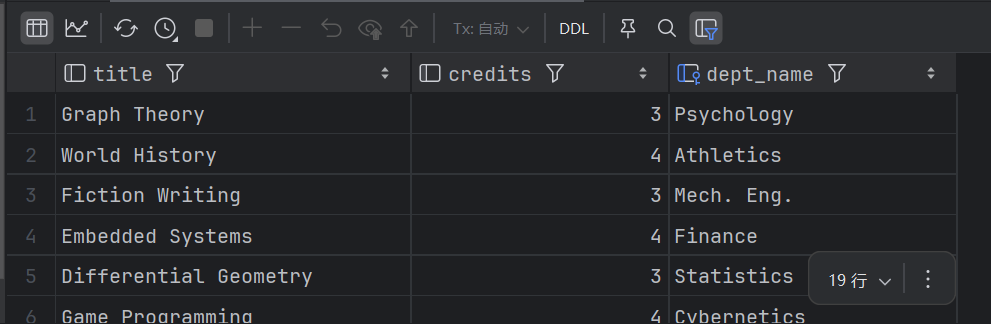
\includegraphics[width=10cm]{./images/20.Question16.png}
    	\caption{Question 16}
    \end{figure}
    
    得到的结果是:(Graph Theory,3,Psychology)等19个元组
    
    \subsubsection{Question 17}
    
    Give the title of the course offered in Chandler during the Fall of 2010.  (medium)
    
    \begin{lstlisting}[language=sql, title=Question 17, tabsize=4]
    	select title
    	from course
    			join section
    				on course.course_id = section.course_id
    	where building = 'Chandler'
    	  and semester = 'Fall'
    	  and year = 2010;
    \end{lstlisting}
    
    运行结果如下图所示:
    
    \begin{figure}[H]
    	\centering
    	
\includegraphics[width=7cm]{./images/21.Question17.png}
    	\caption{Question 17}
    \end{figure}
    
    得到的结果是:International Trade
    
    \subsubsection{Question 18}
    
    List the names and buildings of all departments sorted by the budget from large to small. (medium)
    
    \begin{lstlisting}[language=sql, title=Question 18, tabsize=4]
    	select dept_name, building
    	from department
    	order by budget desc;
    \end{lstlisting}
    
    运行结果如下图所示:
    
    \begin{figure}[H]
    	\centering
    	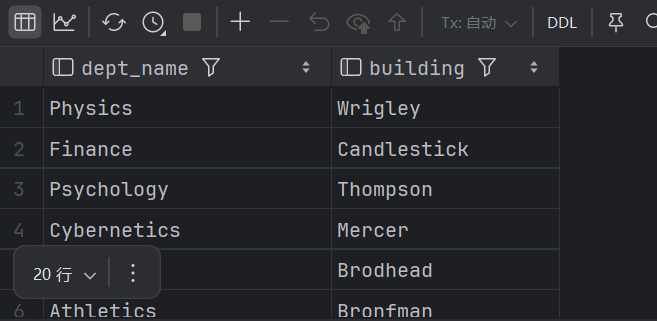
\includegraphics[width=9cm]{./images/22.Question18.png}
    	\caption{Question 18}
    \end{figure}
    
    得到的结果是:(Physics, Wrigley)等20个元组
    
    \subsubsection{Question 19}
    
    Find the names and average salaries of all departments whose average salary is greater than 42000. (medium)
    
    \begin{lstlisting}[language=sql, title=Question 19, tabsize=4]
    	select department.dept_name, avg(salary) as avg_salary
    	from department
    		join instructor
    		on department.dept_name = instructor.dept_name
    	group by department.dept_name
    	having avg_salary > 42000;
    \end{lstlisting}
    
    运行结果如下图所示:
    
    \begin{figure}[H]
    	\centering
    	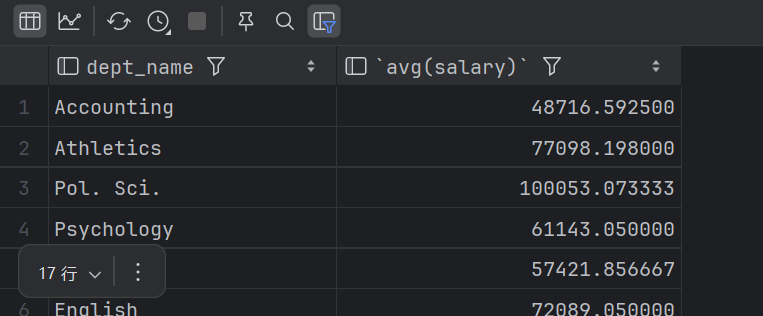
\includegraphics[width=9cm]{./images/23.Question19.png}
    	\caption{Question 19}
    \end{figure}
    
    得到的结果是:(Accounting, 48716.592500)等17个元组
    
    \subsubsection{Question 20}
    
    Find the number of rooms with more than 50 capacity for each building. (medium)
    
    \begin{lstlisting}[language=sql, title=Question 20, tabsize=4]
    	select building, count(*) as num_rooms
    	from classroom
    	where capacity > 50
    	group by building;
    \end{lstlisting}
    
    运行结果如下图所示:
    
    \begin{figure}[H]
    	\centering
    	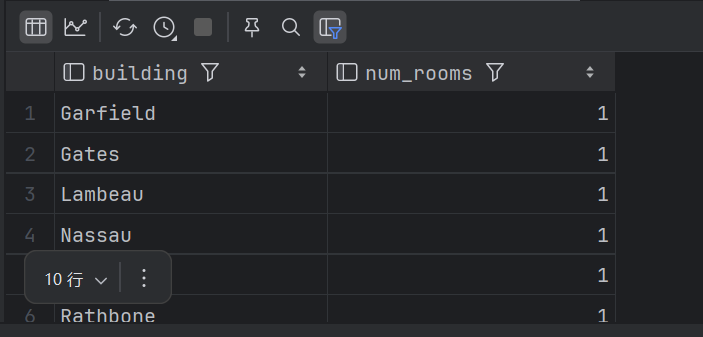
\includegraphics[width=7cm]{./images/24.Question20.png}
    	\caption{Question 20}
    \end{figure}
    
    得到的结果是:11
    
    \subsubsection{Question 21}
    
    Find the total number of students in each department.  (medium)
    
    \begin{lstlisting}[language=sql, title=Question 21, tabsize=4]
    	select department.dept_name, count(student.name) as students_number
    	from department
    			join student
    			on department.dept_name = student.dept_name
    	group by department.dept_name;
    \end{lstlisting}
    
    运行结果如下图所示:
    
    \begin{figure}[H]
    	\centering
    	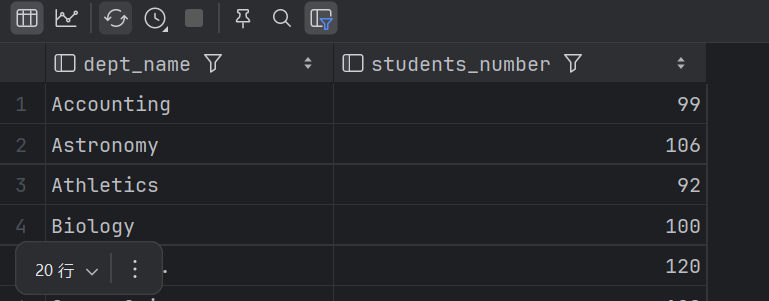
\includegraphics[width=9cm]{./images/25.Question21.png}
    	\caption{Question 21}
    \end{figure}
    
    得到的结果是:(Account, 99)等20个元组
    
    \subsubsection{Question 22}
    
    How many rooms whose capacity is less than 50 does the Lamberton building have?  (medium)
    
    \begin{lstlisting}[language=sql, title=Question 22, tabsize=4]
    	select count(*)
    	from classroom
    	where capacity < 50
    	  and building = 'Lamberton';
    \end{lstlisting}
    
    运行结果如下图所示:
    
    \begin{figure}[H]
    	\centering
    	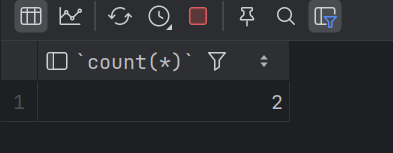
\includegraphics[width=7cm]{./images/26.Question22.png}
    	\caption{Question 22}
    \end{figure}
    
    得到的结果是:2
    
    \subsubsection{Question 23}
    
    What are the names of students who have more than one advisor? (medium)
    
    答案1:\mybox[blue]{假设相同的name表示同一个学生}
    
    \begin{lstlisting}[language=sql, title=Question 23, tabsize=4]
    	select name
    	from student
    			join advisor
    				on student.ID = advisor.s_ID
    	group by name
    	having count(i_ID) > 1;
    \end{lstlisting}
    
    运行结果如下图所示:
    
    \begin{figure}[H]
    	\centering
    	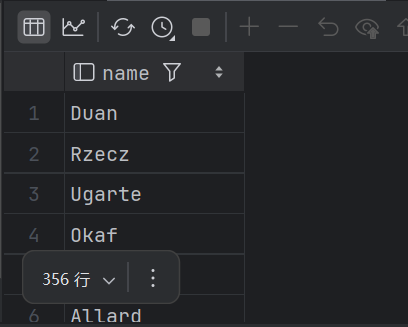
\includegraphics[width=7cm]{./images/27.Question23-ans1.png}
    	\caption{Question 23}
    \end{figure}
    
    得到的结果是:(Duan, 2), (Rzecz, 2)等356 个元组
    
    \mybox[red]{备注:由于本题涉及到了id没有重复值,name却有432个重复值的问题,所以本题上传第二种答案}
    
    答案2:\mybox[blue]{假设相同的ID表示同一个学生}
    
    \begin{lstlisting}[language=sql, title=Question 23, tabsize=4]
    	select ID
    	from student
    			join advisor
    				on student.ID = advisor.s_ID
    	group by ID
    	having count(i_ID) > 1;
    \end{lstlisting}
    
    运行结果如下图所示:
    
    \begin{figure}[H]
    	\centering
    	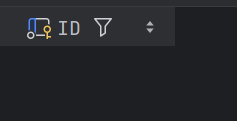
\includegraphics[width=7cm]{./images/27.Question23-ans2.png}
    	\caption{Question 23}
    \end{figure}
    
    得到的结果是:空
    
    \subsubsection{Question 24}
    
    Find the department name of the instructor whose name contains 'Soisalon'. (medium)
    
    \begin{lstlisting}[language=sql, title=Question 24, tabsize=4]
    	SELECT dept_name
    	FROM instructor
    	WHERE name LIKE '%Soisalon%'
    	  OR name LIKE 'Soisalon%'
    	  OR name LIKE '%Soisalon'
    	  OR name = 'Soisalon';
    \end{lstlisting}
    
    运行结果如下图所示:
    
    \begin{figure}[H]
    	\centering
    	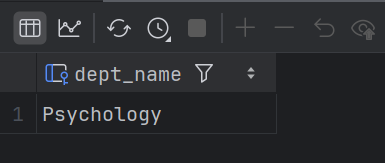
\includegraphics[width=7cm]{./images/28.Question24.png}
    	\caption{Question 24}
    \end{figure}
    
    得到的结果是:Psychology
    
    \subsubsection{Question 25}
    
    Give the name of the department with the lowest budget. (medium)
    
    \begin{lstlisting}[language=sql, title=Question 25, tabsize=4]
    	select dept_name
    	from department
    	order by budget
    	limit 1;
    \end{lstlisting}
    
    运行结果如下图所示:
    
    \begin{figure}[H]
    	\centering
    	
\includegraphics[width=7cm]{./images/29.Question25.png}
    	\caption{Question 25}
    \end{figure}
    
    得到的结果是:Comp. Sci.
    
    \subsubsection{Question 26}
    
    What is the title of the course that is a prerequisite for Mobile Computing?  (hard)
    
    \begin{lstlisting}[language=sql, title=Question 26, tabsize=4]
    	select title
    	from course
    	where course_id in (select prereq_id
    					    from course
    								join prereq
    									on course.course_id = prereq.course_id
    						where course.title = 'Mobile Computing');
    \end{lstlisting}
    
    运行结果如下图所示:
    
    \begin{figure}[H]
    	\centering
    	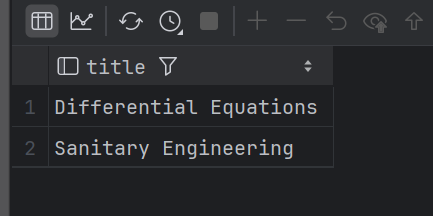
\includegraphics[width=7cm]{./images/30.Question26.png}
    	\caption{Question 26}
    \end{figure}
    
    得到的结果是:Differential Equations, Sanitary Engineering
    
    \subsubsection{Question 27}
    
    What are the names of the 3 departments with the most courses? (hard)
    
    \begin{lstlisting}[language=sql, title=Question 27, tabsize=4]
    	select course.dept_name
    	from department
    			join course
    				on department.dept_name = course.dept_name
    	group by course.dept_name
    	order by count(course_id) desc
    	limit 3;
    \end{lstlisting}
    
    运行结果如下图所示:
    
    \begin{figure}[H]
    	\centering
    	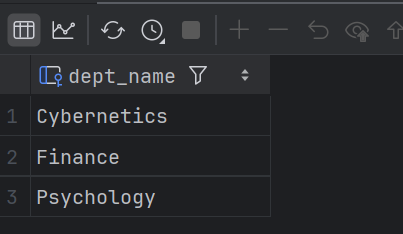
\includegraphics[width=7cm]{./images/31.Question27.png}
    	\caption{Question 27}
    \end{figure}
    
    得到的结果是:Cybernetics, Finance, Psychology
    
    \subsubsection{Question 28}
    
    Find the id of the courses that do not have any prerequisite? (hard)
    
    \begin{lstlisting}[language=sql, title=Question 28, tabsize=4]
    	(select course.course_id
    	 from course)
    	except
    	(select course.course_id
    	 from course
    			join prereq
    				on course.course_id = prereq.course_id);
    \end{lstlisting}
    
    运行结果如下图所示:
    
    \begin{figure}[H]
    	\centering
    	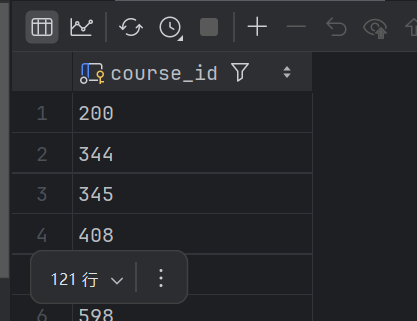
\includegraphics[width=7cm]{./images/32.Question28.png}
    	\caption{Question 28}
    \end{figure}
    
    得到的结果是:200, 344, 345等121个元组
    
    \subsubsection{Question 29}
    
    What are the names of students who took a course in the Fall of 2003?  (hard)
    
    \begin{lstlisting}[language=sql, title=Question 29, tabsize=4]
    	select name
    	from student
    			join takes
    				on student.ID = takes.ID
    	where semester = 'Fall'
    	  and year = 2003;
    \end{lstlisting}
    
    运行结果如下图所示:
    
    \begin{figure}[H]
    	\centering
    	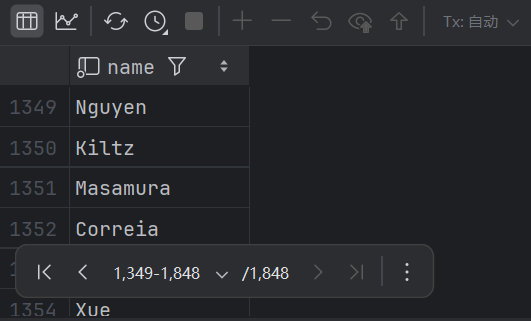
\includegraphics[width=7cm]{./images/33.Question29.png}
    	\caption{Question 29}
    \end{figure}
    
    得到的结果是:Milanic, lindner等1848个元组
    
    \mybox[blue]{还是因为name相同指的是同名还是不同的人,我这里也运行了当作是不同的人的代码(即加上distinct)}
    
    得到的另一个结果是:Milanic, lindner等1093个元组
    
    \subsubsection{Question 30}
    
    Find the semester and year which has the least number of students taking any class.  (hard)
    
    \begin{lstlisting}[language=sql, title=Question 30, tabsize=4]
    	select semester, year
    	from takes
    	group by semester, year
    	order by count(*)
    	limit 1;
    \end{lstlisting}
    
    运行结果如下图所示:
    
    \begin{figure}[H]
    	\centering
    	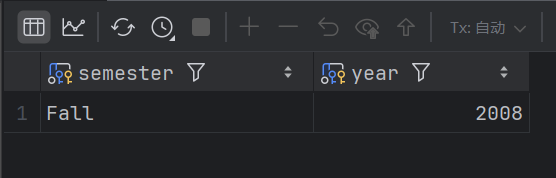
\includegraphics[width=9cm]{./images/34.Question30.png}
    	\caption{Question 30}
    \end{figure}
    
    得到的结果是:Fall, 2008
    
    \subsubsection{Question 31}
    
    Find the id of instructors who didn't teach any courses?  (hard)
    
    \begin{lstlisting}[language=sql, title=Question 31, tabsize=4]
    	(select distinct id
    	 from instructor)
    	except
    	(select distinct instructor.ID
    	 from instructor
    			join teaches
    				on instructor.ID = teaches.ID);
    \end{lstlisting}
    
    运行结果如下图所示:
    
    \begin{figure}[H]
    	\centering
    	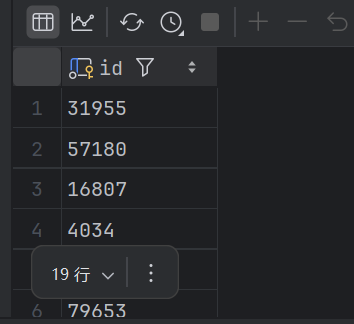
\includegraphics[width=7cm]{./images/35.Question31.png}
    	\caption{Question 31}
    \end{figure}
    
    得到的结果是:Yazdi, Moreira等19个元组
    
    \subsubsection{Question 32}
    
    Find the name of students who took some course offered by Statistics department.  (hard)
    
    \begin{lstlisting}[language=sql, title=Question 32, tabsize=4]
    	select name
    	from student
    			join takes
    				 on student.ID = takes.ID
    			join section
    				 on takes.course_id = section.course_id 
    				and takes.sec_id = section.sec_id 
    				and takes.semester = section.semester and takes.year = section.year
    			join course
    			 	 on section.course_id = course.course_id
    	where course.dept_name = 'Statistics';
    \end{lstlisting}
    
    运行结果如下图所示:
    
    \begin{figure}[H]
    	\centering
    	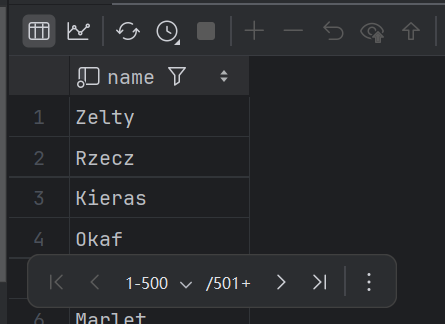
\includegraphics[width=7cm]{./images/36.Question32.png}
    	\caption{Question 32}
    \end{figure}
    
    得到的结果是:Zelty, Rzecz等606个元组

	\mybox[blue]{还是因为name相同指的是同名还是不同的人,我这里也运行了当作是不同的人的代码(即加上distinct)}
	
	得到的另一个结果是:Zelty, Rzecz等515个元组
    
    \subsubsection{Question 33}
    
    What are the titles of courses without prerequisites?  (hard)
    
    \begin{lstlisting}[language=sql, title=Question 33, tabsize=4]
    	(select title
    	 from course)
    	except
    	(select title
    	 from course
    			join prereq
    				on course.course_id = prereq.course_id);
    \end{lstlisting}
    
    运行结果如下图所示:
    
    \begin{figure}[H]
    	\centering
    	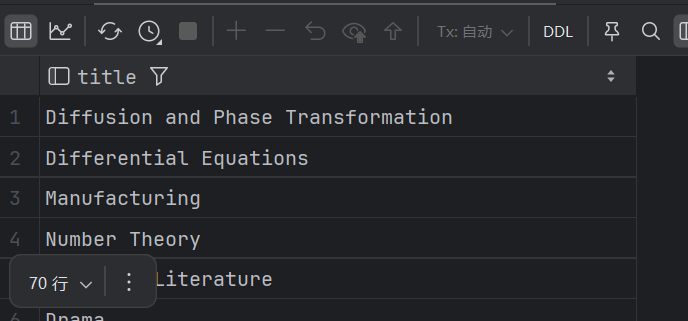
\includegraphics[width=9cm]{./images/37.Question33.png}
    	\caption{Question 33}
    \end{figure}
    
    得到的结果是:Diffusion and Phase Transformation等70个元组
    
    \subsubsection{Question 34}
    
    Find names of instructors with salary greater than that of some (at least one) instructor in the Biology department.  (hard)
    
    \begin{lstlisting}[language=sql, title=Question 34, tabsize=4]
    	select name
    	from instructor
    	where salary > some (select salary
    						 from instructor
    						 where dept_name = 'Biology');
    \end{lstlisting}
    
    运行结果如下图所示:
    
    \begin{figure}[H]
    	\centering
    	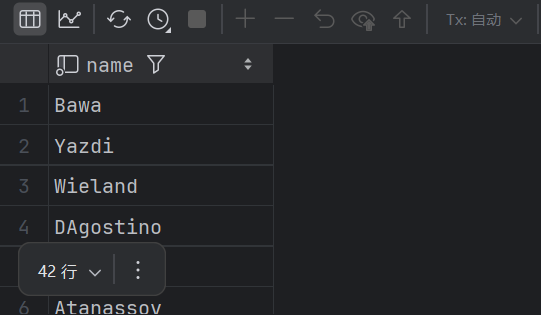
\includegraphics[width=9cm]{./images/38.Question34.png}
    	\caption{Question 34}
    \end{figure}
    
    得到的结果是:(Bawa, 72140.88)等42个元组
    
    \subsubsection{Question 35}
    
    How many instructors are in the department with the highest budget, and what is their average salary?  (hard)
    
    \begin{lstlisting}[language=sql, title=Question 35-1, tabsize=4]
    	select count(*)
    	from instructor
    	where dept_name = (select department.dept_name
    					   from department
    								join instructor
    									on department.dept_name = instructor.dept_name
    					   order by budget desc
    					   limit 1);
    \end{lstlisting}
    
    运行结果如下图所示:
    
    \begin{figure}[H]
    	\centering
    	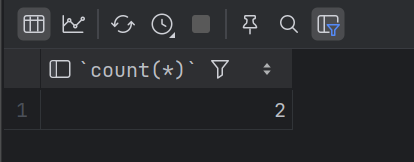
\includegraphics[width=7cm]{./images/39.Question35-1.png}
    	\caption{Question 35-1}
    \end{figure}
    
    \begin{lstlisting}[language=sql, title=Question 35-2, tabsize=4]
    	select avg(salary)
    	from instructor
    	where dept_name = (select department.dept_name
    					   from department
    								join instructor
    									on department.dept_name = instructor.dept_name
    					   order by budget desc
    					   limit 1);
    \end{lstlisting}
    
    运行结果如下图所示:
    
    \begin{figure}[H]
    	\centering
    	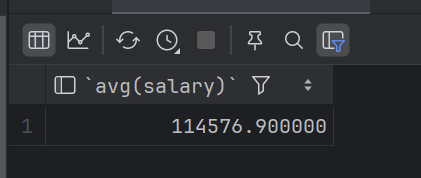
\includegraphics[width=7cm]{./images/40.Question35-2.png}
    	\caption{Question 35-2}
    \end{figure}
    
    得到的结果是:2和114576.900000
    
    \subsubsection{Question 36}
    
    What are the names of students who haven't taken any Biology courses?  (hard)
    
    \begin{lstlisting}[language=sql, title=Question 36, tabsize=4]
    	(select distinct name
    	 from student)
    	except
    	(select distinct name
    	 from student
    			join takes
    				on student.ID = takes.ID
    	 where dept_name = 'Biology');
    \end{lstlisting}
    
    运行结果如下图所示:
    
    \begin{figure}[H]
    	\centering
    	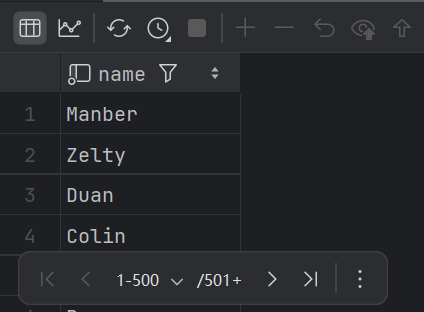
\includegraphics[width=7cm]{./images/41.Question36.png}
    	\caption{Question 36}
    \end{figure}
    
    得到的结果是:Manber, Zelty, Duan等1469个元组
    
    \subsubsection{Question 37}
    
    Give the title of the prerequisite to the course International Finance.  (hard)
    
    \begin{lstlisting}[language=sql, title=Question 37, tabsize=4]
    	select title
    	from course
    	where course_id = (select prereq_id
    					   from course
    								join prereq
    									on course.course_id = prereq.course_id
    					   where title = 'International Finance');
    \end{lstlisting}
    
    运行结果如下图所示:
    
    \begin{figure}[H]
    	\centering
    	
\includegraphics[width=7cm]{./images/42.Question37.png}
    	\caption{Question 37}
    \end{figure}
    
    得到的结果是:Elastic Structures
    
    \subsubsection{Question 38}
    
    What is the name of the department with the most credits?  (hard)
    
    \begin{lstlisting}[language=sql, title=Question 38, tabsize=4]
    	select department.dept_name
    	from department 
    			join course
    				on department.dept_name = course.dept_name
    	group by department.dept_name
    	order by sum(credits) desc
    	limit 1;
    \end{lstlisting}
    
    运行结果如下图所示:
    
    \begin{figure}[H]
    	\centering
    	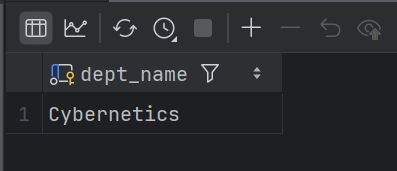
\includegraphics[width=7cm]{./images/43.Question38.png}
    	\caption{Question 38}
    \end{figure}
    
    得到的结果是:Cybernetics
    
    \subsubsection{Question 39}
    
    Give the name and building of the departments with greater than average budget.  (extra)
    
    \begin{lstlisting}[language=sql, title=Question 39, tabsize=4]
    	select dept_name, building
    	from department
    	where budget > (select avg(budget)
    	from department);
    \end{lstlisting}
    
    运行结果如下图所示:
    
    \begin{figure}[H]
    	\centering
    	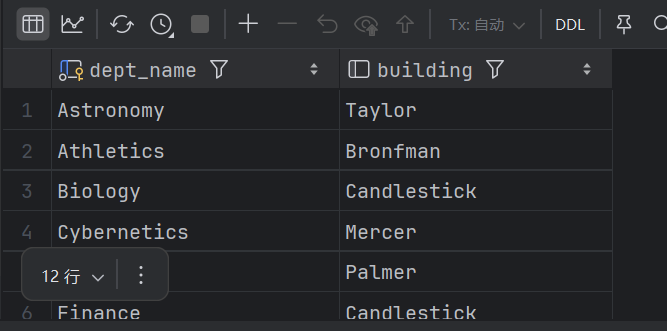
\includegraphics[width=9cm]{./images/44.Question39.png}
    	\caption{Question 39}
    \end{figure}
    
    得到的结果是:(Astronomy, Taylor)等12个元组
    
    
    \section{存在的问题及解决方案}
    
    \subsection{存在的问题:}
    
    在实验开始阶段,由于表格数量较多,且表格之间都有较强的关联性,一次性理解所有表格之间的关联有着一定的难度,为了防止在完成问题的时候需要很多次翻阅表格之间的关系和表格的内容,将表格之间的关系绘制成了关系图谱。
    
    \subsection{解决方案:}
    
    绘制了如图2和图13的两张关系图谱,且在两张表格之间的连接线上写出了连接的关系(实际上是join的时候on部分所需要验证的条件)这样可以用图形化界面清晰地展示表格之间的关系,方便解答问题。这样一来,在做题的方便程度和流畅度上都有了明显的提升。
    
    \section{实验小结}
    
    通过本次实验的完成,我对关系型数据库中的数据查询、表间关系操作等知识点有了更深入的理解。
    
    \begin{itemize} 
    	\item \textbf{深入理解表间关系的意义和操作}:实验过程中通过绘制关系图谱,进一步加深了对数据库表结构及其内在关联的理解,尤其在涉及多表查询及复杂条件筛选时,图谱极大降低了操作复杂性。
    	
    	\item \textbf{熟悉了SQL语句的高级运用}:本次实验中,利用了如\texttt{JOIN}、\texttt{GROUP BY}、子查询、聚合函数等多种SQL语句和操作,解决了具有挑战性的复杂查询问题。
    	
    	\item \textbf{提高了效率与规范性}:通过提前梳理表结构,解决了实验初期因表格较多、关系复杂带来的效率问题,保证了实验的完整性和流畅性。
    	
    	\item \textbf{问题分析与解决能力的提升}:实验涉及多个难度不一的问题,通过将问题分解并逐步优化解决方案,比如将“大于平均值”拆分为“查询平均值”和“大于指定值”两个问题来解决,极大的简化了解题难度,不仅锻炼了解题能力,还积累了处理SQL问题的经验。
    \end{itemize}
    
    本次实验让我对关系型数据库及SQL查询操作的运用有了更加全面的认识和技能提升,为后续复杂数据库操作打下了良好的基础。
\end{document}
